%%%%%%%%%%%%%%%%
%%% PROBLEM EXTENSIONS
%%%%%%%%%%%%%%%%
\section{PROBLEM EXTENSIONS}



%%%%%%%%%%%%%%%%
%%% PER PROVINCE/TERRITORY FLP
%%%%%%%%%%%%%%%%
\subsection{Per Province/Territory FLP}
Wind turbine waste management is a problem faced by all Canadian Provinces. We limited the scope of this to Ontario however, most decommissioned wind turbine blades in Canada are landfilled due to health concerns and a lack of wind turbine recycling facilities to cope with supply \cite{RN12}  \cite{RN1}.  Due to the growth in the number of turbines and the catastrophic environmental impact of landfilling, all provinces are looking to recycle turbine blades and preserve the environment.  Consequently, a natural extension of both the facility location and routing problems would be to solve these for each province.  

We will only investigate the wind turbine facility location problem (FLP) for each Canadian Province, as is the most pressing issue for policymakers \cite{RN14}. The recycling facilities are crucial for recycling the blades, whereas the recycling trucks are not as limiting. By diverting the fiberglass from landfills in each province, Canada can be a global leader in wind turbine recycling while developing a new supply of rare earth metals, critical minerals, and fibreglass to meet global demand \cite{RN17}.

The per-province FLP has the same problem description and formulation as in section \ref{section:problem_desc} while following the same data standardization process explained in subsection \ref{subsection:dataset_description}. However, the implementation is limited to wind farms within the defined borders of each province. The optimization performs one province at a time. We generated the locations of recycling facilities and optimal numbers for each province. The results are displayed in Figure \ref{fig:fig_pbp} below. 

\begin{figure} [h]
    \centering
    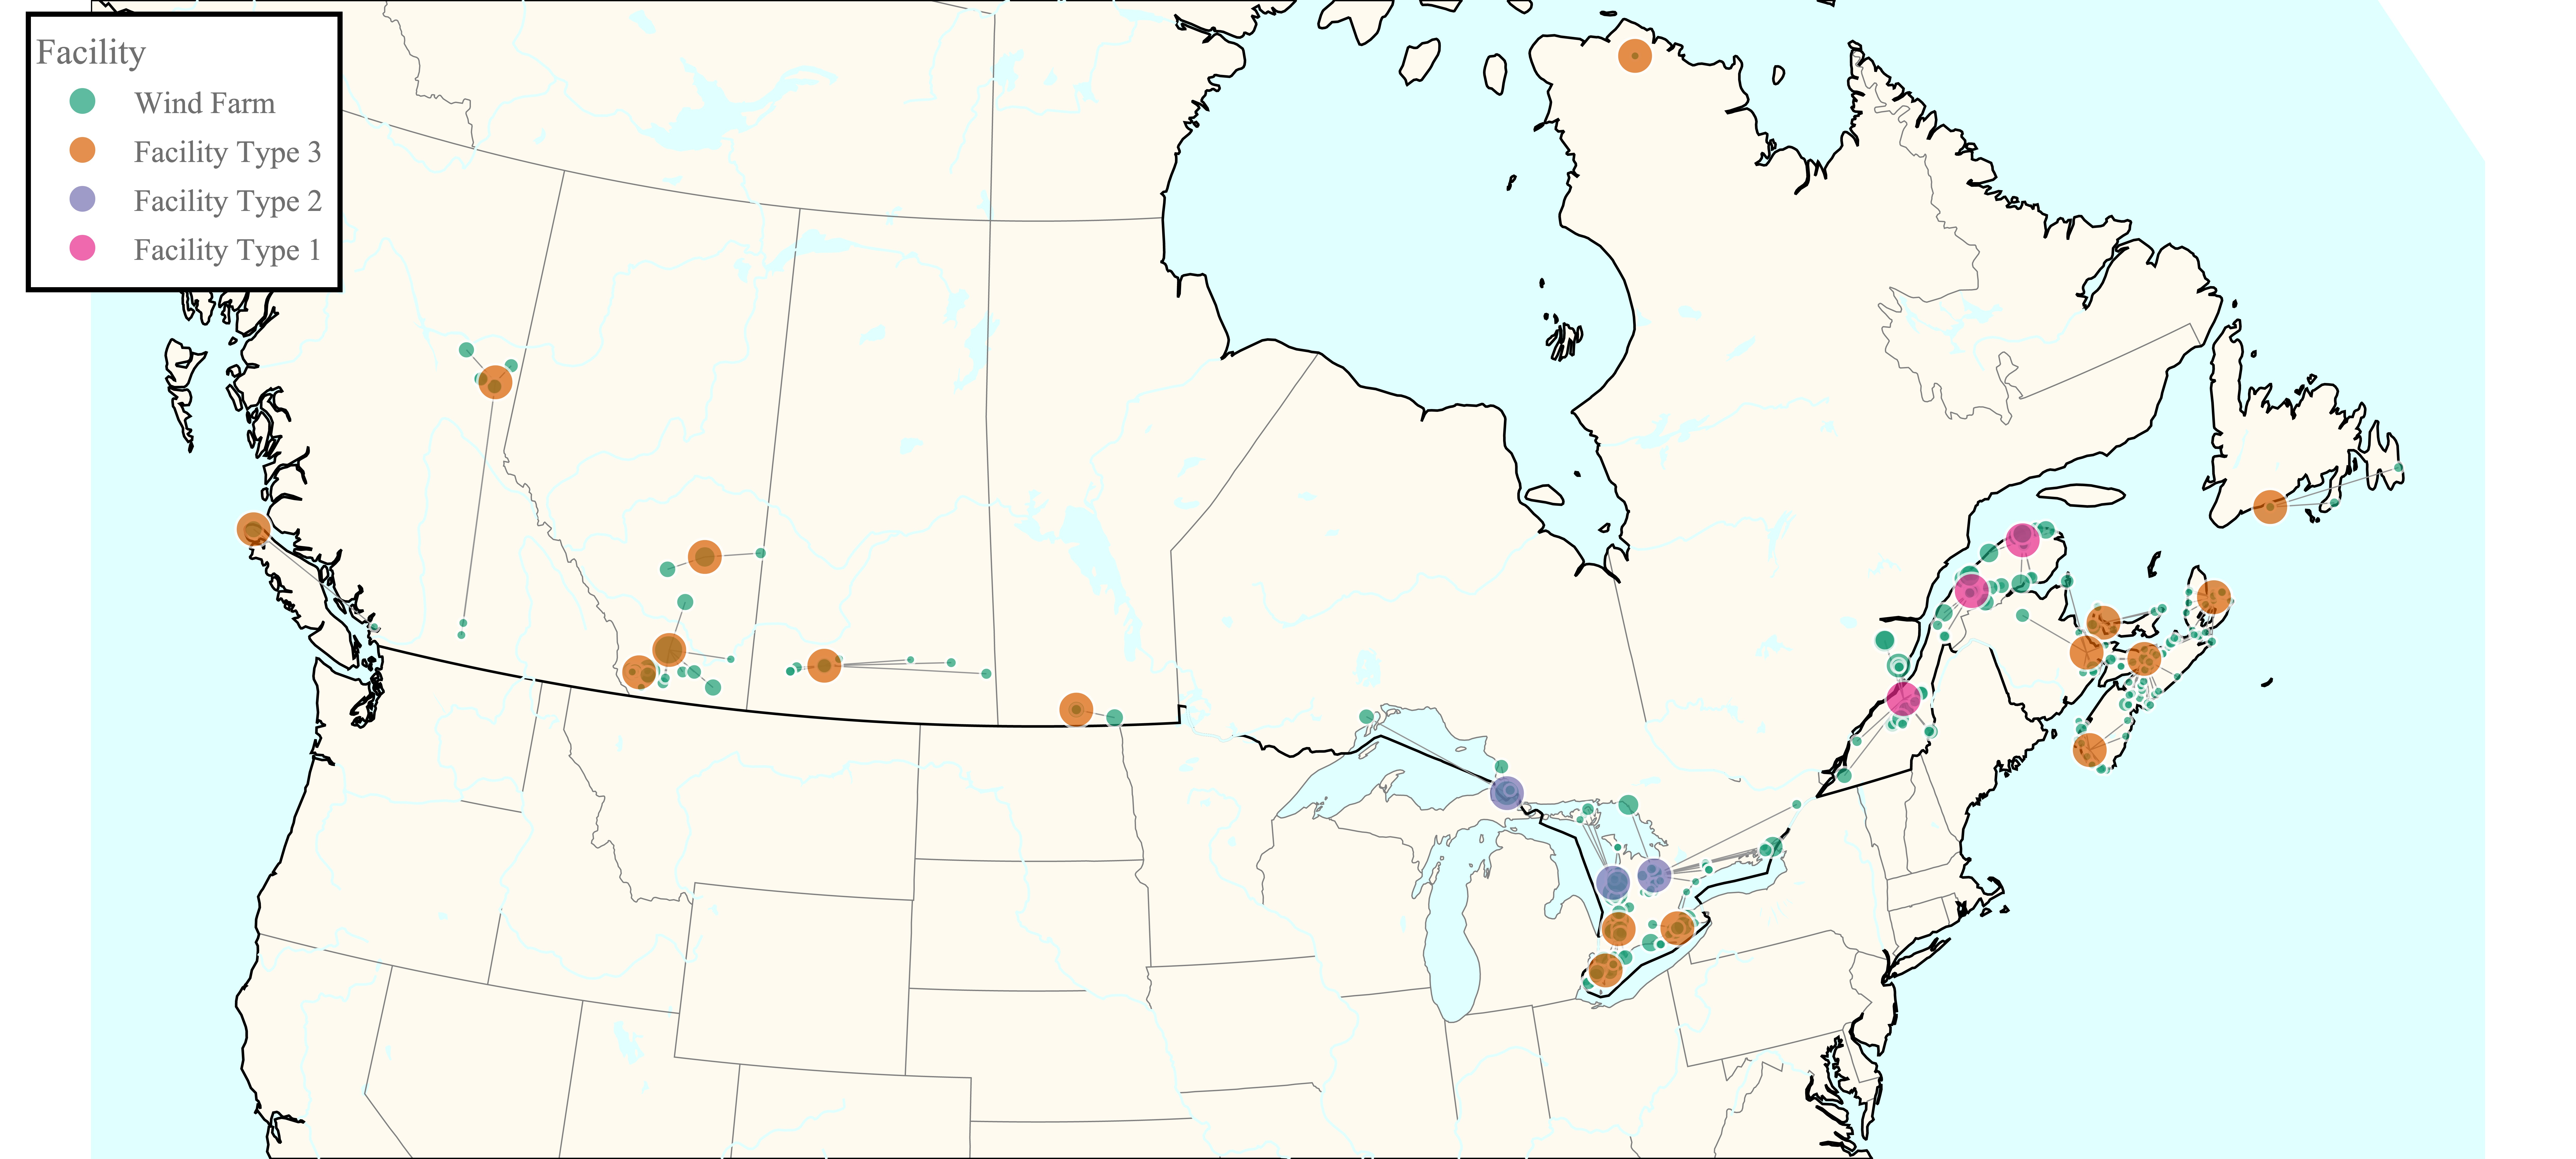
\includegraphics[width=0.9\textwidth]{graphics/fig_pbp.jpeg}
    \caption{Per Province/Territory FLP}
    \label{fig:fig_pbp}
\end{figure}

The resulting problem generated the following solution: 22 recycling facilities in Canada, 3 of Type 1, 3 of Type 2, and  16 of Type 3. The cost of delivery over 50 years is \$100 million with a total building cost of \$87.78 million. The total is approximately \$187.8 million.  

There are some limitations to this approach. First Canada is one of the largest countries by land, with unique geographic features, therefore some locations while mathematically optimal may not make practical sense. For instance, having recycling facilities in the northern territories may be invalid, because of geographic isolation for raw materials or lack of transportation. A second limitation is that we have not built in a function for additional pricing when changing transportation methods.  For instance, having a facility on the northern tip of Vancouver Island implies that the blades are loaded onto trucks then boats, which will certainly have associated costs. Therefore this location may not be as beneficial as something closer to the southern wind turbines in British Columbia, especially considering the mountainous terrain the blades would have to otherwise traverse.


%%%%%%%%%%%%%%%%
%%%FEDERAL FLP : PAN-CANADIAN OPTIMIZATION
%%%%%%%%%%%%%%%%
While we may have solved the FLP at the provincial level, the limitations of Canadian geography are a crucial consideration. Some wind farms would be better served by recycling facilities outside of their province. In fact, in the Maritimes or western Ontario, some wind farms are closer to neighboring provinces, and the cost could be reduced by sending the blades shorter distances outside of their province. Let’s assume that the federal government has nationalized this industry to meet environmental goals by 2050. In this alternate timeline, they control the subsidies and want to reduce the total amount of fixed and transportation costs. The TSP portion of this extension will not be examined as it is not an immediate legislative concern for Canada 2.0. 

In view of this problem extension, we aim to eliminate the assumption that the waste generated by a wind farm must be recycled in the same province as the wind farm. This should centralize the waste distribution and reduce the total fixed cost. Since each facility can source from a larger supply pool, they will be much closer to maximum capacity, instead of having spare capacity from the per-province mode.  

To model this assumption in our FLP, we will update our dataset by adding the wind farms from all Canadian Provinces and Canadian Territories excluding offshore wind farms, and null values briefly mentioned in the data cleaning subsection. Offshore wind farms are not considered in this FLP because the logistical requirements to recycle offshore wind farm turbines are different from land wind farms.  

We followed the same data standardization process explained in subsection \ref{subsection:dataset_description} of this paper while adding the wind farms from all Canadian Provinces to the dataset. In addition, all the assumptions, formulations and constraints developed in section \ref{section:problem_desc} are valid except for the one bounding recycling to local provinces. The optimal location results are displayed in figure \ref{fig:fig_can} below. 

\subsection{Federal FLP: Pan-Canadian Optimization}
\begin{figure} [h]
    \centering
    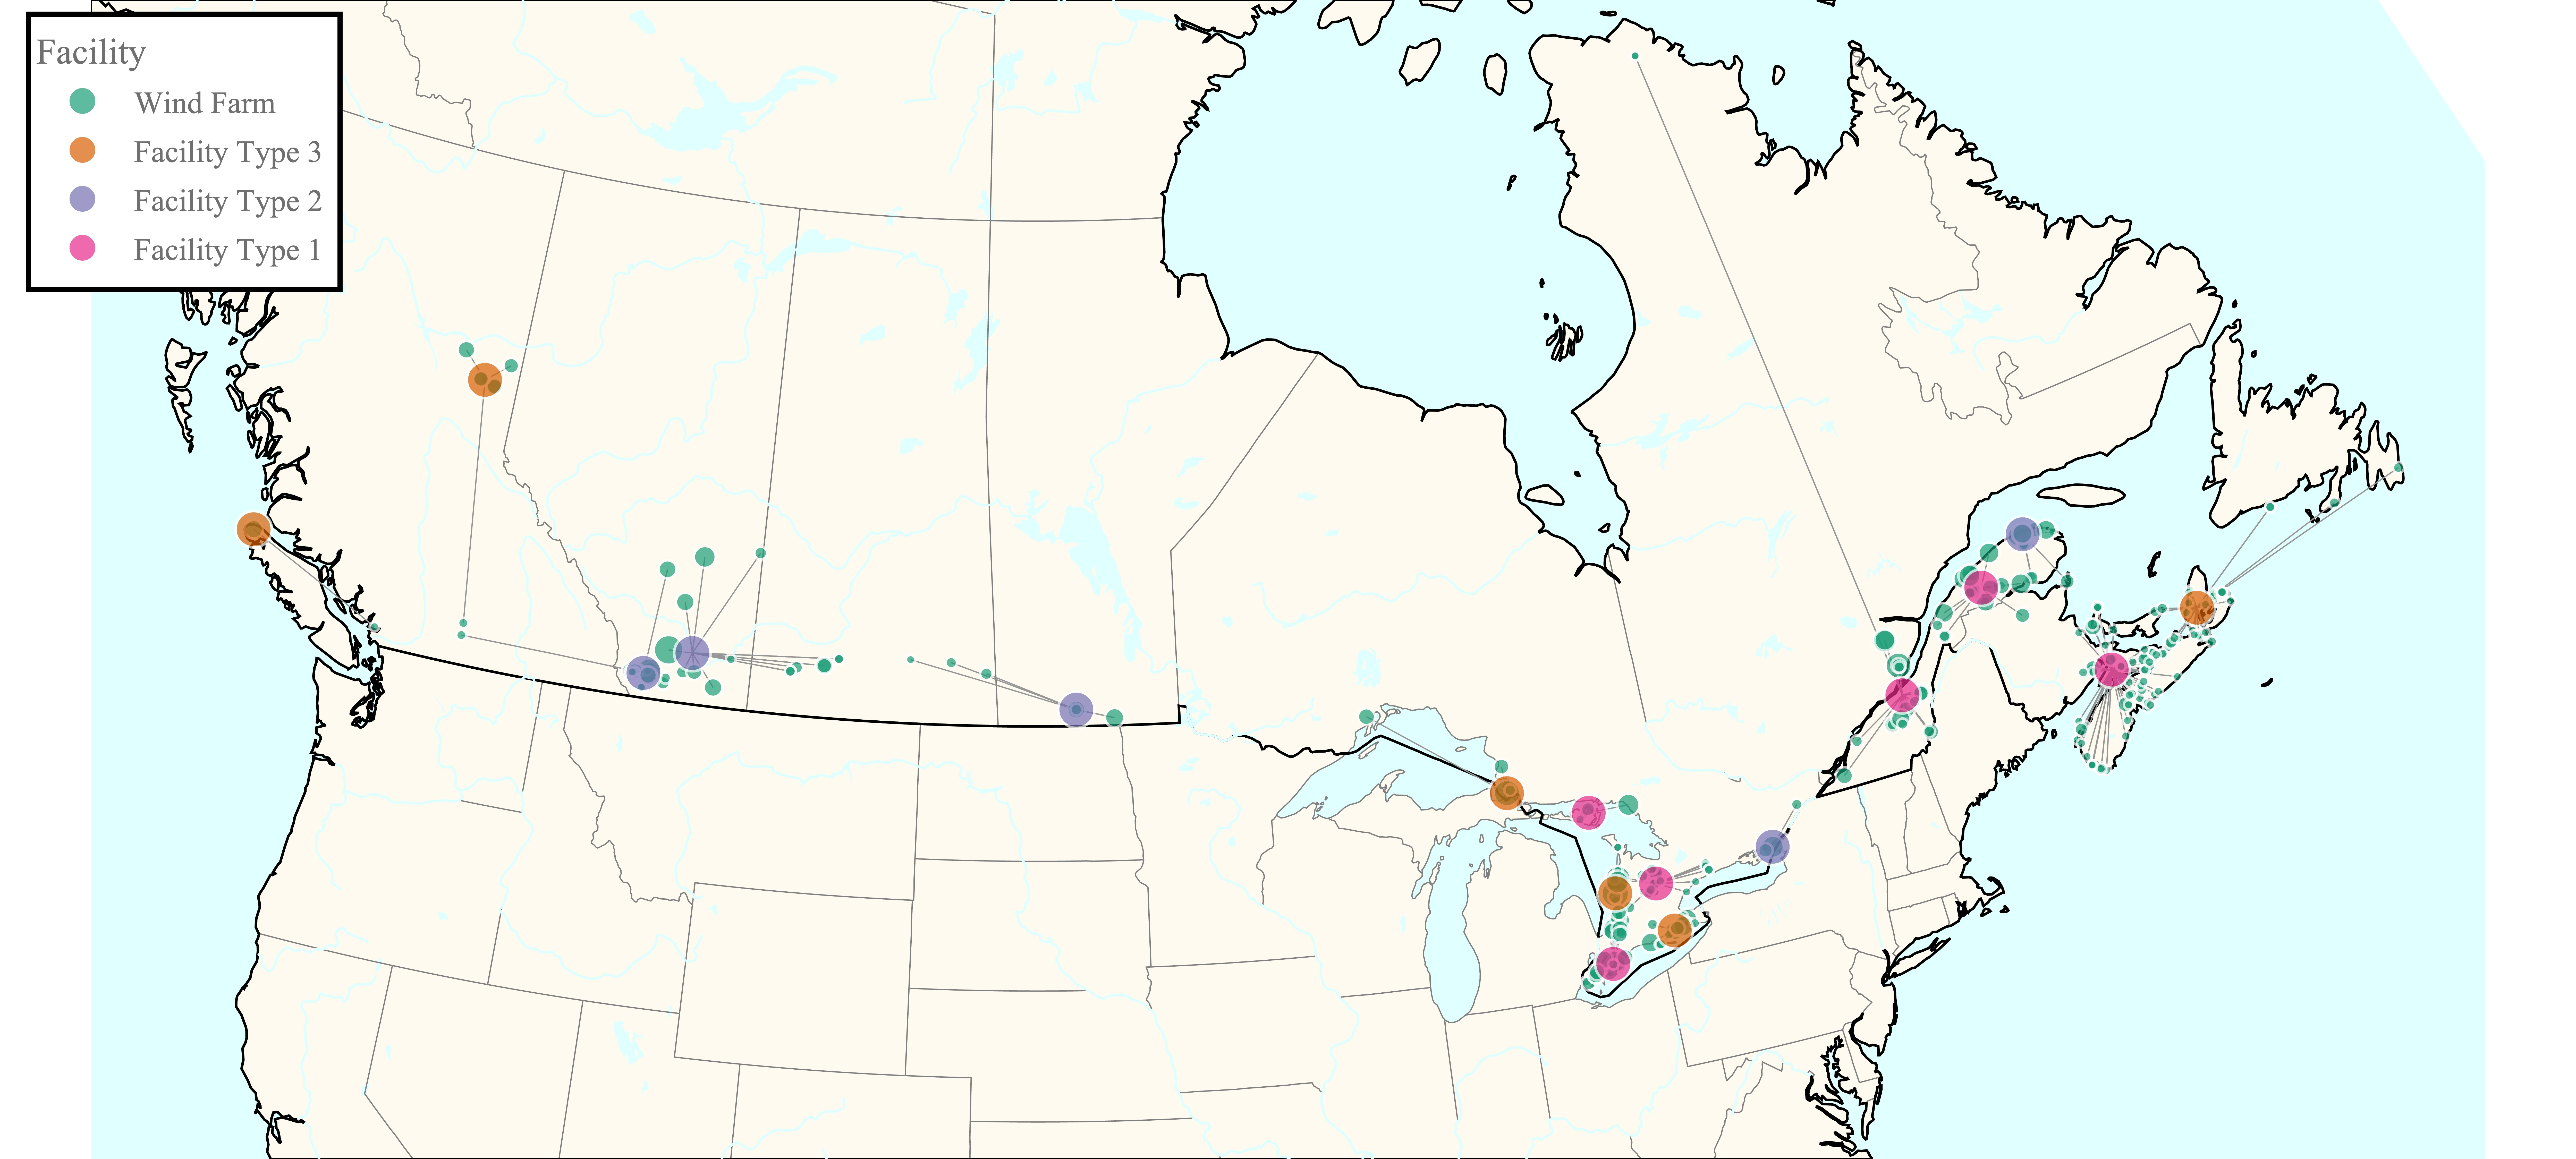
\includegraphics[width=0.9\textwidth]{graphics/fig_can.jpeg}
    \caption{Federal FLP: Pan-Canadian Optimization}
    \label{fig:fig_can}
\end{figure}

The result of the Federal FLP are the following one: 16 recycling facilities accross Canada, 6 of Type 1, 5 of Type 2, and 6 of Type 3. The cost of delivery over 50 years is \$130.33 million and the cost of building facilities is \$78.54 million. The total is therefore \$208.87 million over 50 years. This Federal FLP is far more expensive than the Per Province/Territory FLP due to delivery costs. There may be several explanations for this, however the two most likely are that the Gurobi code is limited by computational power and time. Additional optimal solutions may exist and can be solved with additional time, but we were unable to run the model for unlimited time. Furthermore, this model formulation theoretically prioritizes maximum capacity over minimum distance, as the loads from windfarms are not split and therefore the model prioritizes fixed cost savings (\$78 million vs \$87 for provincial). These limitations are best addressed with additional runtime and constraints. 



%%%%%%%%%%%%%%%%
%%%YEAR-BY-YEAR EXTENSION
%%%%%%%%%%%%%%%%
\subsection{Year-by-year extension}
With the current solution approach, we are ignoring the “lumpy” characteristic of turbine waste. Generally, all the wind blades within a wind farm must be replaced within a few years of each other. Depending on the year, there might be a significant amount of waste or none. With our current approach, there is no such “lumpy” characteristic, as we assume the supply is evenly spread over a long period. The current simplification of the facility location problem allows for efficient computational time and an approximate solution. However, the year-by-year deliveries of waste would look very different from our model and from a realistic case. 

To make the model more realistic, it is possible to extend the model by the addition of a ‘time’ index. Instead of using average annual waste, we can approximate yearly waste of wind turbines. This would allow us to better approximate real-world conditions via this formulation. By adding a $T$ set, indicating a specific year within our planning horizon we could modify our $dw$ decision variable, our demand and capacity constraints, and our objective as follows: 
%\vspace{-10pt}
\begin{equation}
    dw_{wfty} - \text{integer variable indicating how many deliveries to make from } w \text{ to } f,t \text{ in year } y
\end{equation}
\vspace{-10pt}
\begin{equation}
    \sum_{f,t} dw_{wfty} = wd_{wy} \quad \forall wy \quad \quad \text{Demand}
\end{equation}
\vspace{-10pt}
\begin{equation}
    \sum_{w} dw_{wfty} * ww_{w} \le ca_{t} * fb_{ft} \quad \forall wyt \quad \quad \text{Capacity}
\end{equation}
\vspace{-10pt}
\begin{equation}
    \sum_{wtfy} (dist_{wft} * dw_{wfty} * dc * dk) \quad \quad \text{Objective}
\end{equation}

While this addition brings the model closer to real-world conditions, expanding the problem with a time index makes the problem significantly more difficult and computationally challenging to solve. As such we would recommend splitting the problem into two phases, similarly to our current formulation. In phase 1 locating the facility locations through the average annual delivery is acceptable as the facilities have a much longer useful life than the wind farms and can reach a steady state at some point in their lifetime. Then phase 2 decides how to distribute the waste between facilities with a time index, to better represent the “lumpy” supply which may be solved as a larger instance of the problem. Additionally by having a time index, we would be able to better link the two models, by only allowing the wind blade waste to be delivered after wind blades haves been cut.